\chapter{Implementazione Hardware}
\label{chap:implementazione_hardware}
\section{Tecnologie di base}

In questo capitolo tratteremo tutte le tecnologie utilizzate nel progetto, come i microcontrollori e i dispositivi di output,
 concentrandoci sull’ESP32.

\subsection{Panoramica dell’ESP32}

\subsubsection{Generalità}
I microcontrollori (MCU) sono circuiti integrati che combinano nello stesso chip un microprocessore con una serie di componenti periferici
 come: memoria, timer, convertitori analogico-digitali e soprattutto pin di I/O.

A differenza di un microprocessore (CPU), i microcontrollori non sono pensati per svolgere onerose attività di calcolo ma per interagire 
il più possibile con l’ambiente esterno, gestendo numerosi scambi fra le periferiche di Input/Output.

L’ESP32, sviluppato da Espressif Systems, rappresenta un microcontrollore avanzato con architettura dual-core Tensilica LX6 a 32 bit
 (alcune varianti hanno anche core single-core o LX7), integrando al suo interno Wi-Fi e Bluetooth a basso consumo. Questa caratteristica
  lo rende particolarmente adatto per applicazioni IoT (Internet of Things), domotica e sistemi embedded complessi (Espressif, 2024 \cite{Espressif2024}).

\subsubsection{Famiglie di ESP32}
I microcontrollori sono suddivisi in famiglie a seconda del processore e delle periferiche integrate. Nel caso dell’ESP32,
 troviamo diverse varianti come ESP32-WROOM-32, ESP32-WROVER, ESP32-C3, ESP32-S2 ed ESP32-S3.  
Queste versioni condividono la stessa architettura di base ma differiscono per risorse di memoria, numero di GPIO disponibili,
 supporto a periferiche aggiuntive o funzionalità avanzate come acceleratori AI.  

La scelta del modulo da utilizzare deve essere fatta non sulla base delle prestazioni massime, ma dell’ottimalità rispetto al
 progetto in questione (Patti, 2024 \cite{Patti2024}).

\subsubsection{Componenti hardware}
Ogni ESP32 integra al suo interno non solo la CPU, ma anche le memorie e una grande quantità di periferiche digitali e analogiche, 
oltre ai moduli di comunicazione wireless (Wi-Fi 802.11 b/g/n e Bluetooth 4.2/5.0).  
Questa elevata integrazione consente di ridurre i costi, semplificare il design e garantire maggiore velocità di accesso ai dati.

\begin{figure}[h]
\centering
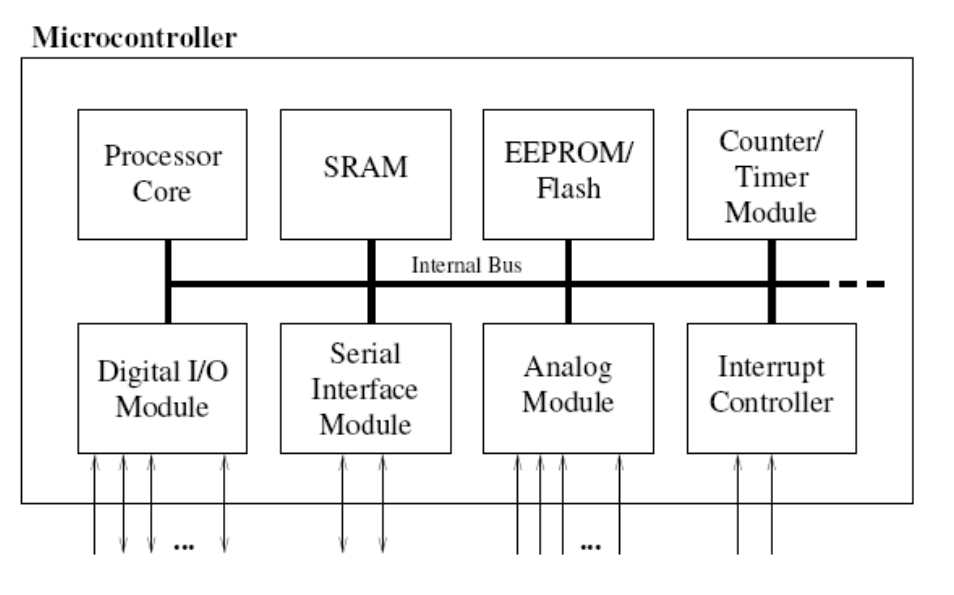
\includegraphics[width=0.7\textwidth]{esp32_block_diagram.png}
\caption{Componenti hardware principali di un microcontrollore ESP32.}
\label{fig:esp32-mcu}
\end{figure}

\subsubsection{Memorie}
Le memorie di un microcontrollore possono essere di tipo volatile e non volatile. Le volatili includono SRAM e DRAM; le non volatili comprendono ROM, EEPROM, Flash e, in alcuni casi, NVRAM.

L’ESP32 tipicamente dispone di:
\begin{itemize}
    \item 448 KB di ROM, che contiene il bootloader e alcune librerie di base;
    \item 520 KB di SRAM interna, divisa tra cache, stack e heap per le applicazioni;
    \item Flash esterna fino a 16 MB (a seconda del modulo), utilizzata per memorizzare codice e file system;
    \item opzionalmente, PSRAM esterna fino a 8 MB, utile per applicazioni che richiedono elaborazioni multimediali o server web embedded.
\end{itemize}

Rispetto ad altre schede, l’ESP32 si distingue per la disponibilità di memoria e per la presenza di connettività wireless integrata, rendendolo una soluzione più completa per progetti IoT e sistemi embedded avanzati (Patti, 2024 \cite{Patti2024}; Espressif, 2024 \cite{Espressif2024}).

